\begin{figure}
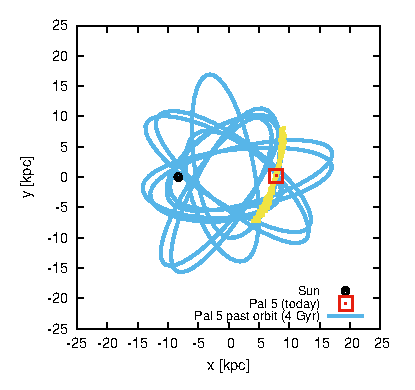
\includegraphics[width=83mm]{./figures/pal5_orbit.eps}\\
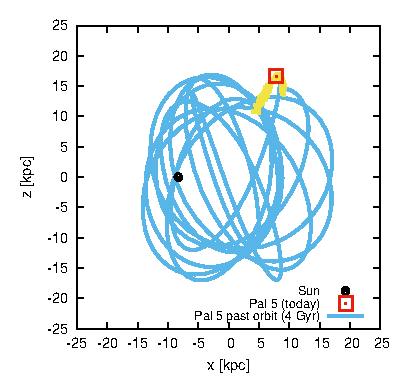
\includegraphics[width=83mm]{./figures/pal5_orbit_xz.eps}
  \caption{Orbit of the Pal\,5 mock within the Milky Way-like potential (Sec.~\ref{sec:challenge}).}
  \label{plot_pal5_orbit}
\end{figure}

\begin{figure*}
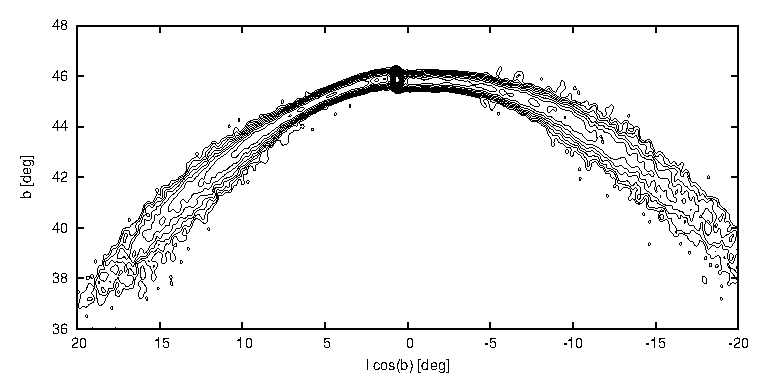
\includegraphics[width=168mm]{./figures/pal5_contour.eps}\\
  \caption{Contour density map of the Pal\,5 mock as seen from the position of the Sun (Sec.~\ref{sec:challenge}).}
  \label{plot_pal5_contour}
\end{figure*}

Most authors have shown that their methods work for simple cases of spherically symmetric galaxy potentials. Here we want to compare performances of different methods in a more realistic potential. The potential we use has the minimum complexity needed to model a disk galaxy like the Milky Way. Moreover, since it is the only prominent stream with a known progenitor and continuous detection over several degrees on the sky, we test our methods with a mock model of Pal\,5, resembling its present-day position, velocity and extent (see \citealt{Kupper15} for a detailed description of the Pal\,5 system).

To generate a Pal\,5-like stream, we ran a direct $N$-body simulation of a low-mass globular cluster, and let it dissolve in a static, Milky Way-like background potential (see Sec.~\ref{ssec:potential}). The model initially consisted of 65,356 single-mass particles of about $0.5\msun$ each, and was evolved for 4\,Gyr using the publicly available code \textsc{Nbody6} \citep{Aarseth03, Nitadori12}. The initial mass of the cluster was $31090\msun$ and it lost $17940\msun$ into the tidal tails, leaving the cluster with a present-day mass of $13150\msun$. The stream therefore consists of roughly 35000 stars.

The orbit of the cluster was chosen such that its present-day position, distance and radial velocity match the observed values for Pal\,5. The position in observable coordinates is RA\,$ = 229.0$\,deg, Dec\,$ = -0.1114$\,deg or $l = 0.8521$\,deg, $b = 45.86$\,deg. Its distance was set to $d_{Sun} = 23.2$\,pc \citep{Harris96}, and the radial velocity to $-58.7$\,km\,s$^{-1}$ \citep{Odenkirchen02}. The proper motion was then chosen such that the profile of the resulting stream matches roughly the observed morphology of Pal\,5 within our choice of galactic potential. The values are $\mu_{\alpha\cos(\delta)}=-2.537$\,mas\,yr$^{-1}$ and $\mu_\delta = -2.649$\,mas\,yr$^{-1}$.

The observables were turned into Cartesian coordinates assuming a Solar galactocentric distance of 8.33\,kpc and a LSR motion of 239.5\,km\,s$^{-1}$ \citep{Gillessen09}. The Solar reflex motion was assumed to be $(11.1, 12.24, 7.25)$\,km\,s$^{-1}$ \citep{Schonrich10}. With these specifications, the present-day Cartesian coordinates of the progenitor in the galactic rest frame are 
\begin{eqnarray}
  (x, y, z) &=& (7816.1,  240.02,  16640)\,\mbox{pc}\\
  (v_x, v_y, v_z) &=& (-37.457, -151.79, -21.610)\,\mbox{km\,s}^{-1}
\end{eqnarray}

The Challenge can be found on the wiki page of the Gaia Challenge workshop\footnote{\url{http://astrowiki.ph.surrey.ac.uk/dokuwiki/doku.php?id=tests:streams:challenges}}, and we invite everyone to download the Challenge and contribute to this comparison project. The columns are described in the header of the file, and more details can be found on the wiki. The columns give Cartesian coordinates and observables for positions and velocities of all particles. All numbers are either in pc and km\,s$^{-1}$, or degree and mas\,yr$^{-1}$, respectively. 



\subsection{The potential}\label{ssec:potential}

We evolve the cluster for 4\,Gyr in a three-component galactic potential consisting of a spherical bulge, a disk and an axissymmetric dark-matter halo. Assuming that we can constrain the disk and bulge potentials better through other sorts of tracers within those components, we are going to fix the disk and bulge parameters in all modeling attempts, and only leave the halo parameters free. 

The functional form of the potential components is as follows. The bulge is modeled as a \citet{Jaffe83} spheroid, 
\begin{equation}
  \Phi_{Bulge}(r) = \frac{GM_{Bulge}}{b_{bulge}}\ln\left(\frac{r}{r+b_{bulge}}\right),
\end{equation}
with $M_{Bulge} = 3.4\times 10^{10}\msun$ and $b_{Bulge} = 700.0$\,pc. The disk component is represented by a \citet{Miyamoto75} potential,
\begin{equation}
  \Phi_{Disk}(r) = -\frac{GM_{Disk}}{\sqrt{R^2+\left(a_{Disk}+\sqrt{z^2+b_{Disk}^2}\right)^2}},
\end{equation}
where $R = \sqrt{x^2+y^2}$, and with $M_{Disk} = 1.0\times 10^{11}\msun$, $a_{Disk} = 6500$\,pc and $b_{Disk} = 260$\,pc. Lastly, we chose a flattened \citet{Navarro97} potential for the dark-matter halo component, 
\begin{equation}
  \Phi_{Halo}(R, z) = -\frac{GM}{\sqrt{R^2+\frac{z^2}{q_z^2}}}\ln\left(1+\frac{\sqrt{R^2+\frac{z^2}{q_z^2}}}{r_{Halo}} \right),
\end{equation}
with $M_{Halo} = 1.81194\times 10^{12}\msun$, $r_{Halo} = 32260$\,pc, and $q_z = 0.814$.

This potential has a nearly flat rotation curve within the disk, with a circular velocity of about 249\,km\,s$^{-1}$ at the assumed position of the Sun. However, the circular velocity at the Solar circle is not the only possible way for comparing modeling results with input values. Below is a list of interesting points at which the quality of the models can be conveniently assessed. Circular velocities are
\begin{itemize}
  \item $V_C(r_{Sun}, 0, 0) = 249.01$\,km\,s$^{-1}$,
  \item $V_C(\vec{r}_{Pal5}) = 247.84$\,km\,s$^{-1}$,
  \item $V_C(r_{Halo}, 0, 0) = 251.99$\,km\,s$^{-1}$,
 \end{itemize}
 and corresponding accelerations are 
 \begin{itemize}
  \item $a(r_{Sun}, 0, 0) = 7.95\,\mbox{pc\,Myr}^{-2}$,
  \item $a(\vec{r}_{Pal5}) = 3.51\,\mbox{pc\,Myr}^{-2}$,
  \item $a(r_{Halo}, 0, 0) = 2.06\,\mbox{pc\,Myr}^{-2}$.
\end{itemize}
